\subsection{Tres patrones observados en el baseline}
\paragraph{Falsos positivos de baja retrodispersión.}
En \texttt{Pakistan\_70625}, las manchas oscuras a la izquierda y arriba reciben alta
probabilidad aunque la referencia solo marca cauces estrechos. Hay 28\,116 FP y
3\,330 FN; la IoU es 0.0408. La mediana VV/VH de los FP es $-17.84/-25.82$ dB,
frente a $-9.07/-17.93$ dB en verdaderos negativos. La señal de los FP se parece a
la del agua correctamente detectada ($-18.01/-26.03$ dB). Esto evidencia ambigüedad
radiométrica en el chip. Superficies lisas o sombra de radar son explicaciones físicas
posibles~\cite{sarhandbook}, pero aquí no se demuestra cuál opera: faltan cobertura,
topografía y una referencia óptica independiente.

\paragraph{Omisión de agua con respuesta más alta.}
En \texttt{Pakistan\_849790}, la referencia marca gran parte del chip como agua,
mientras la predicción retiene principalmente las regiones oscuras. Hay 138\,480 FN
y 793 FP, con recall 0.1945 e IoU 0.1936. La mediana VV/VH de los FN es
$-9.09/-17.90$ dB; la de los TP, $-16.31/-24.80$ dB. El modelo omite agua etiquetada
cuya respuesta difiere de la del agua oscura. Vegetación inundada, rugosidad o doble rebote
pueden cambiar la respuesta SAR~\cite{sarhandbook}; no se identifican esos mecanismos
únicamente por VV/VH. También deben considerarse incertidumbre de anotación y adquisición.

\paragraph{Fragmentación y bordes de cauces estrechos.}
En \texttt{Bolivia\_379434}, el cauce sinuoso derecho presenta bandas próximas de FP y FN
y tramos discontinuos. Se omite además una mancha central de agua. El chip tiene 5\,588 FP,
6\,528 FN e IoU 0.2602. El 81.25\% de los 12\,116 errores cae en una banda de borde
definida por dilatación/erosión binaria de la referencia con tres iteraciones.
Esa concentración apoya un problema de detalle espacial; no demuestra un desplazamiento
global de registro. Las transformaciones imagen/máscara fueron verificadas y se exportó
sin remuestrear. Resolución efectiva, contexto del encoder y definición del límite son
hipótesis adicionales, que deberían contrastarse con recortes y referencias independientes.

Los tres casos fueron inspeccionados técnicamente y registrados en
\texttt{qualitative\_cases.csv}; requieren revisión editorial del grupo.
Los patrones pueden coexistir y sus conteos no representan categorías causales mutuamente
excluyentes. No se afirma que una imagen oscura sea necesariamente agua o sombra.
\begin{figure}[H]\centering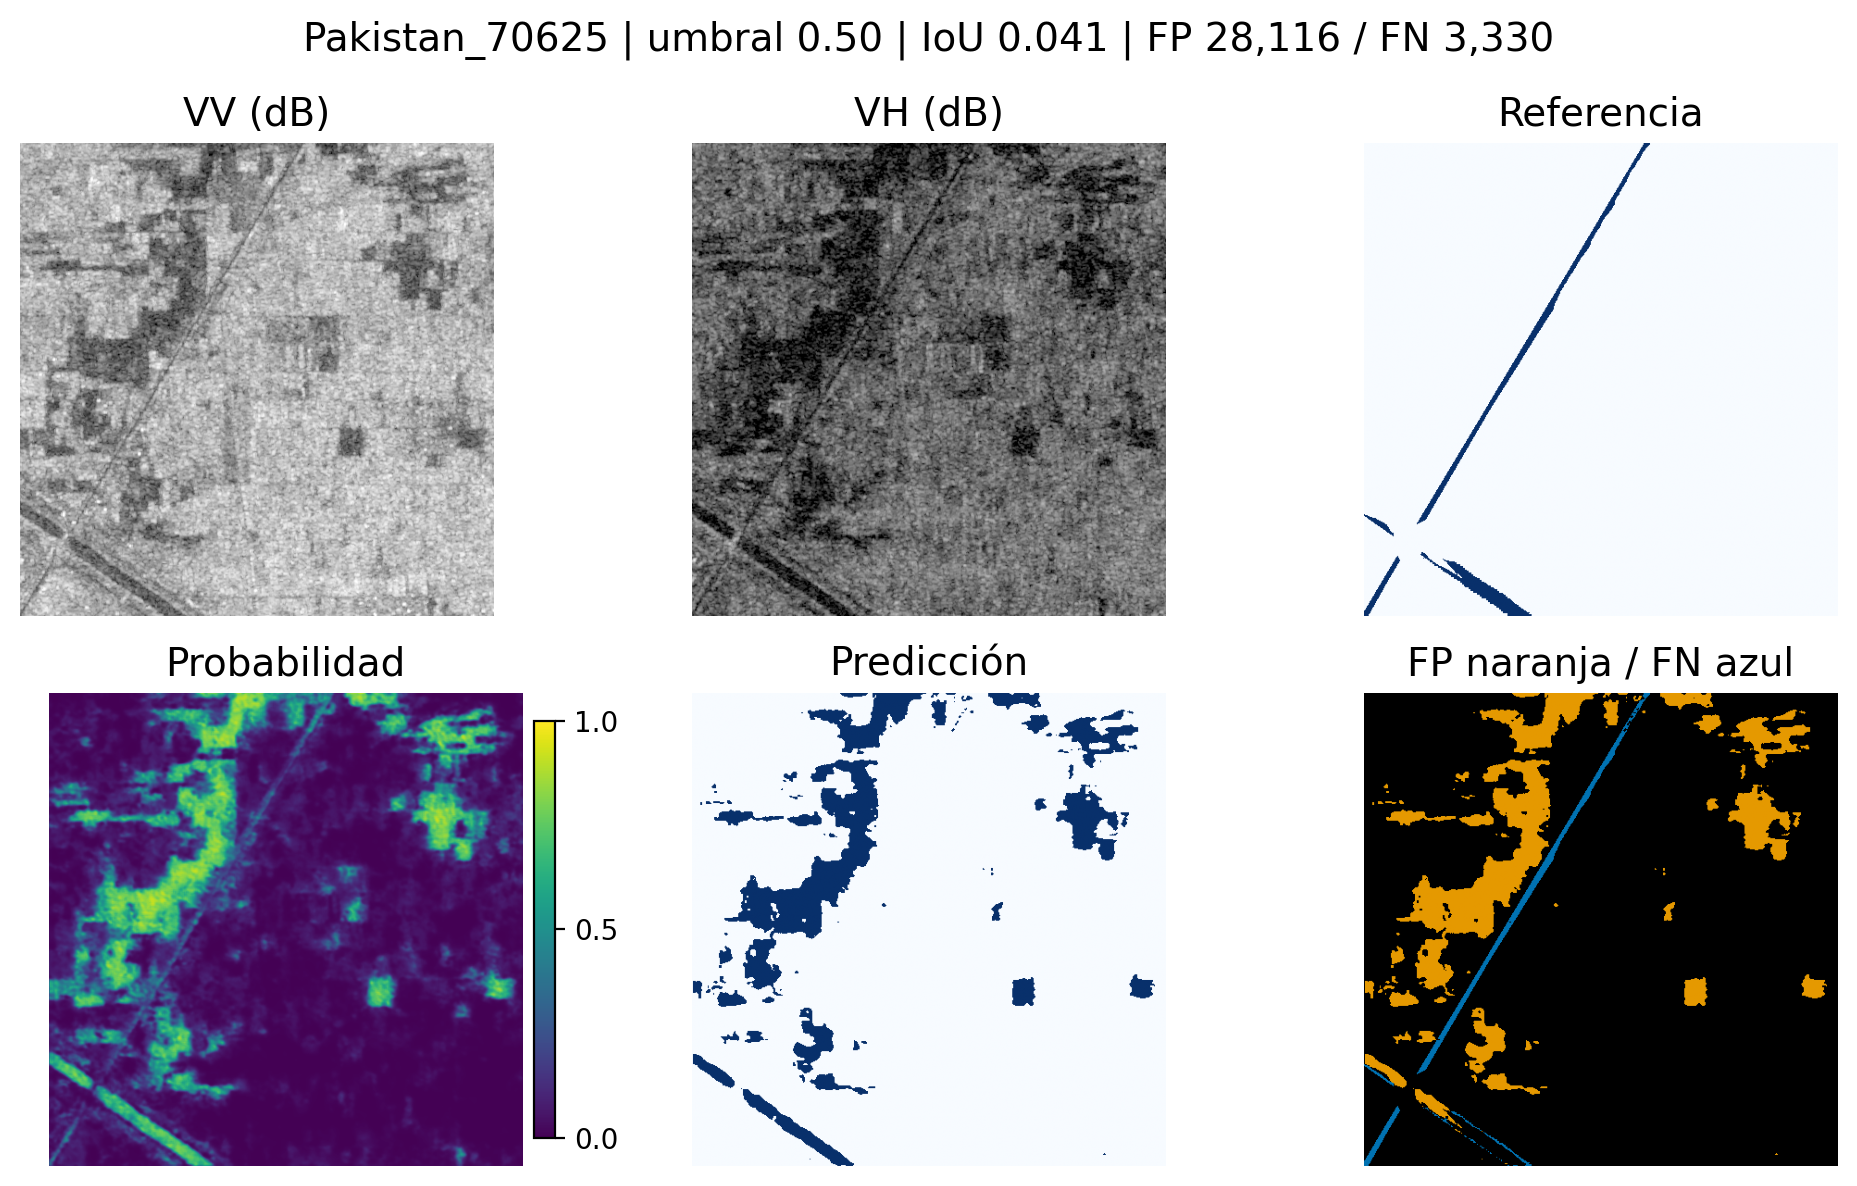
\includegraphics[width=0.96\linewidth]{figures/flood_3.png}\caption{Pakistan\_70625 (test): Se predicen manchas extensas en zonas oscuras sin agua en la referencia; el cauce diagonal fino queda parcialmente omitido.}\end{figure}
\begin{figure}[H]\centering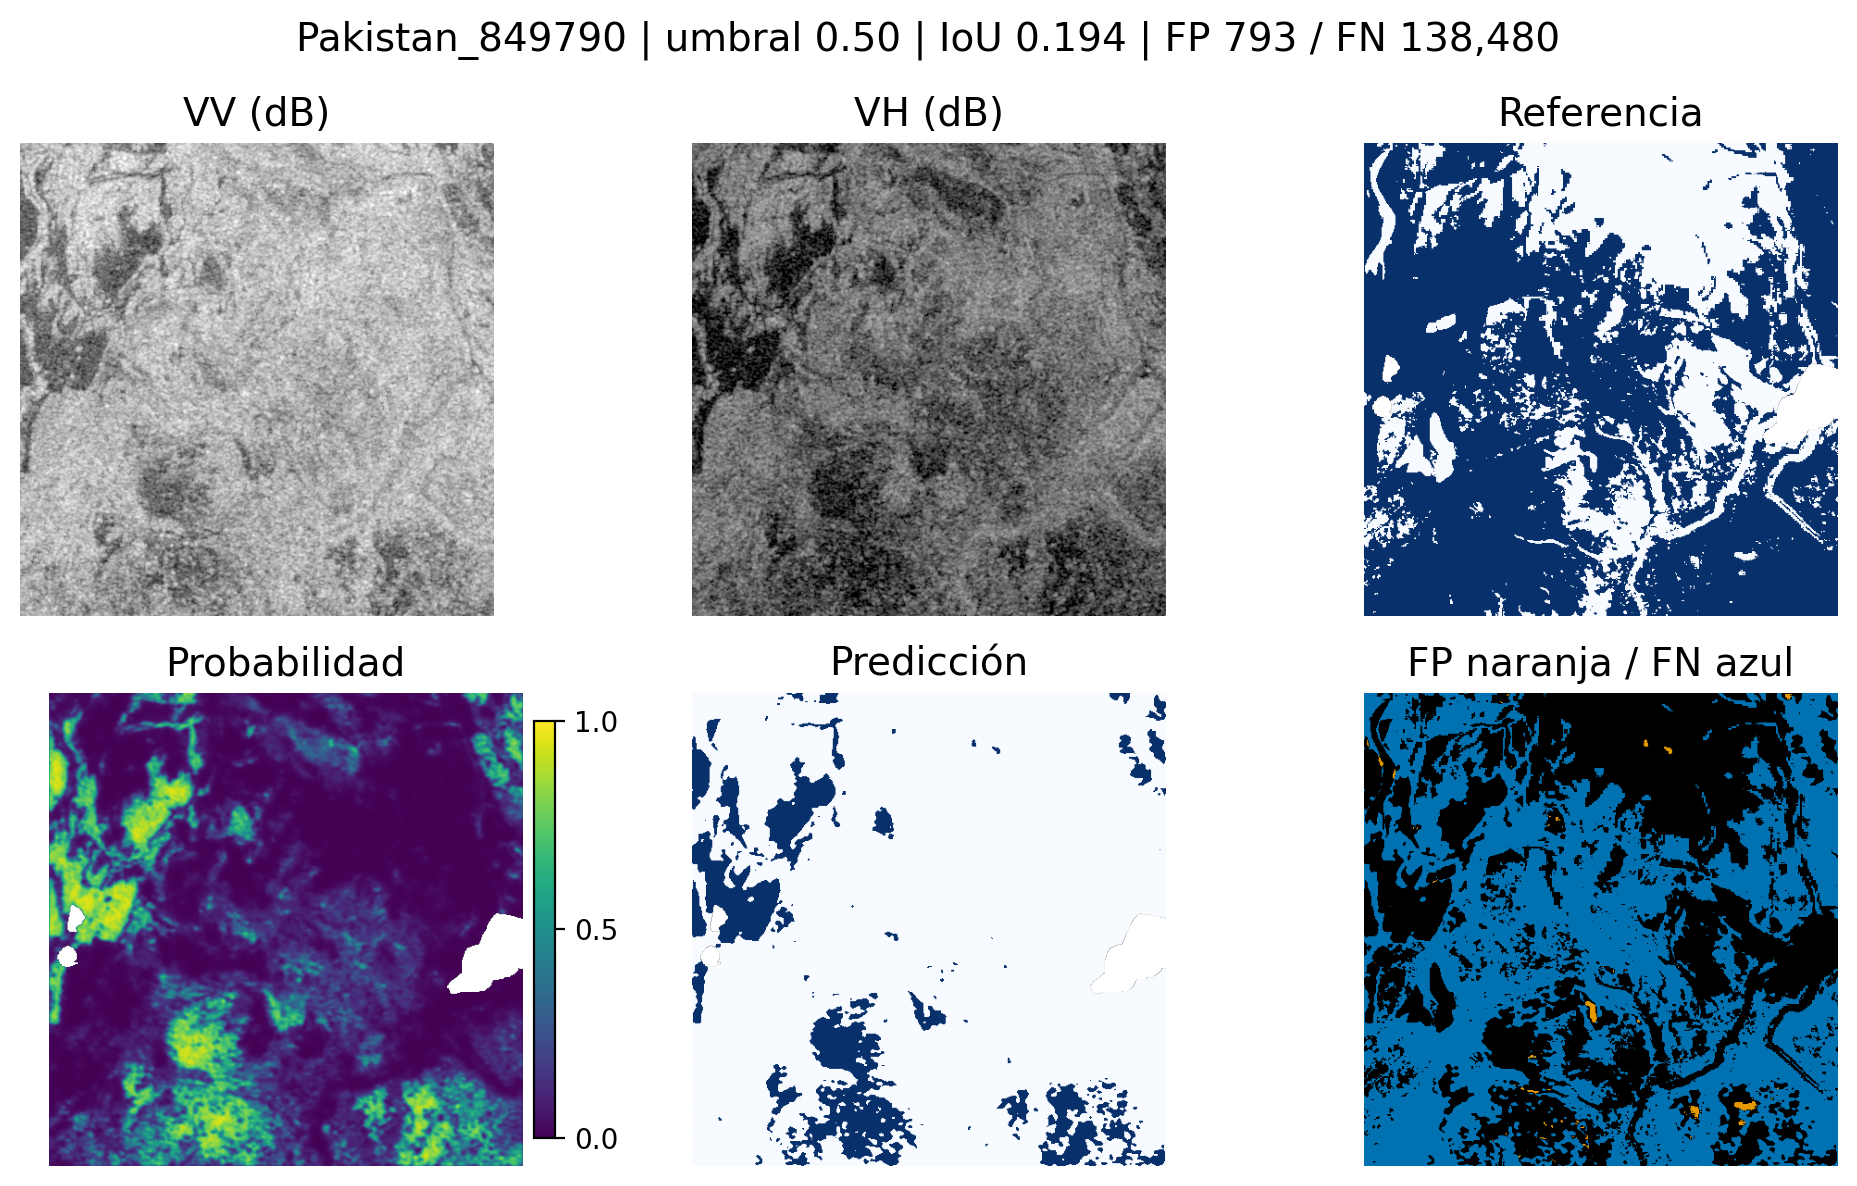
\includegraphics[width=0.96\linewidth]{figures/flood_4.png}\caption{Pakistan\_849790 (test): La referencia cubre gran parte del chip pero la predicción retiene pocas zonas oscuras; predominan falsos negativos en superficies de respuesta más alta.}\end{figure}
\begin{figure}[H]\centering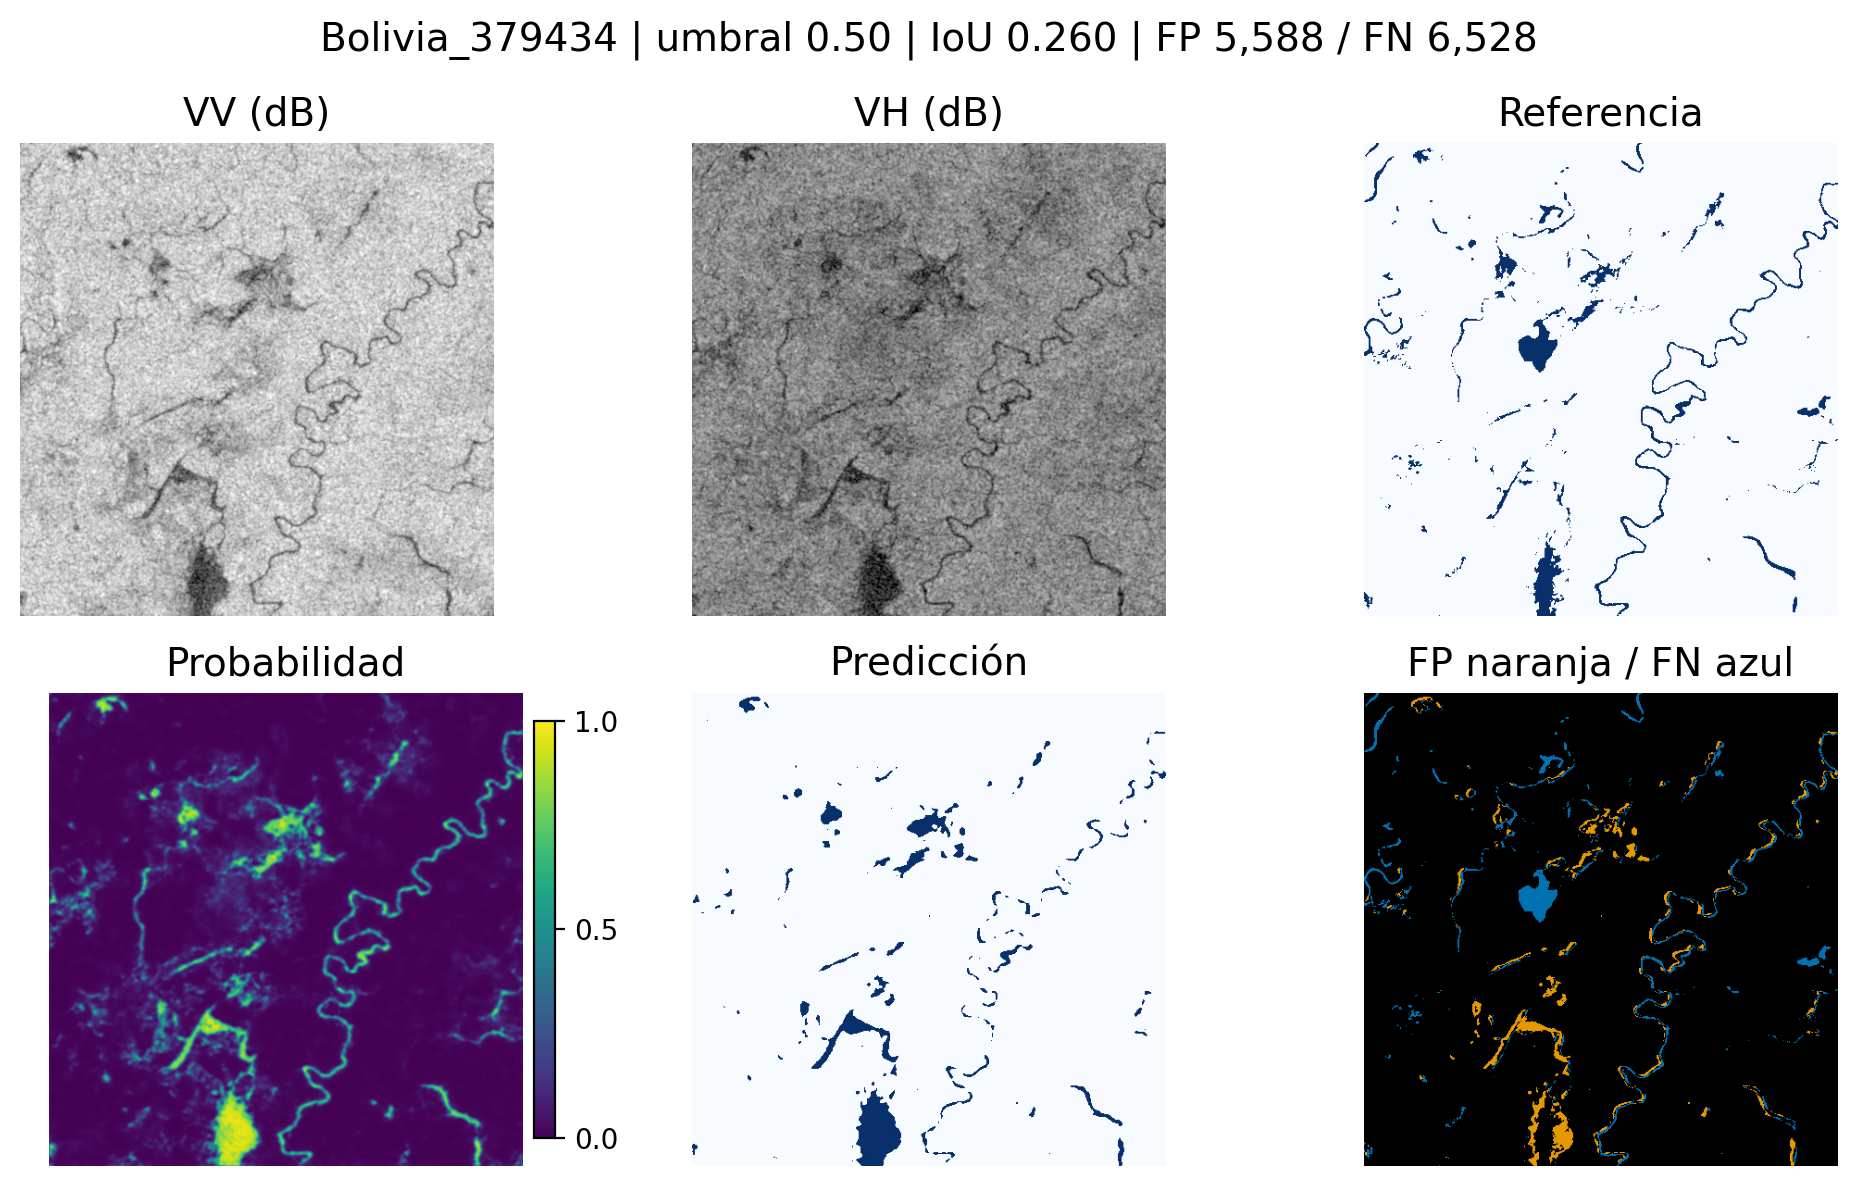
\includegraphics[width=0.96\linewidth]{figures/flood_5.png}\caption{Bolivia\_379434 (bolivia): En el cauce sinuoso derecho aparecen bandas cercanas de FP y FN y tramos fragmentados; también se omite una mancha central de agua.}\end{figure}

\subsection{Dos hipótesis de generalización}
\paragraph{H1: cambia la distribución de apariencia y prevalencia del agua.}
Bolivia tiene 16.00\% de agua válida, frente a 12.30\% en prueba ID y 9.55\% en entrenamiento.
Diferentes proporciones de agua abierta, canales y agua de respuesta alta pueden cambiar
precisión, recall e IoU. Los ejemplos muestran que la respuesta del agua no es uniforme.
Un test de esta hipótesis separaría resultados por cobertura, amplitud VV/VH y tamaño de
regiones, usando anotaciones independientes. La prevalencia medida es evidencia descriptiva;
no demuestra por sí sola una causa de la brecha.

\paragraph{H2: cambian adquisición y sesgo de etiquetas débiles.}
Los metadatos oficiales ubican Bolivia en órbita descendente relativa 156, el 15 de febrero
de 2018. También hay adquisiciones descendentes en entrenamiento, por ejemplo India,
Pakistán y Paraguay; por ello, la dirección descendente no explica por sí sola una diferencia externa.
El número de órbita relativo y la geometría local podrían modificar la señal, pero no
se dispone del ángulo de incidencia por chip. Además, las etiquetas débiles derivadas
de umbralización SAR pueden reforzar la asociación entre agua y baja retrodispersión.
Para contrastarlo se necesitarían geometría/incidencia, cobertura y una comparación con
presupuesto igual de pasos, múltiples semillas y máscaras manuales adicionales.
Bolivia representa un evento externo pequeño; una brecha positiva o negativa no aísla
un efecto geográfico y no permite generalizar a todos los países.
